\documentclass[12pt,a4paper]{article}

% Packages
\usepackage[margin=1in]{geometry}
\usepackage{graphicx}
\usepackage{tikz}
\usetikzlibrary{automata, positioning, arrows.meta}
\usepackage{listings}
\usepackage{xcolor}
\usepackage{hyperref}
\usepackage{fancyhdr}
\usepackage{booktabs}
\usepackage{float}
\usepackage{amsmath}
\usepackage{enumitem}
\usepackage{colortbl}

% Code listing style
\definecolor{codebg}{RGB}{248,248,248}
\definecolor{codeframe}{RGB}{200,200,200}
\definecolor{keyword}{RGB}{0,0,180}
\definecolor{comment}{RGB}{0,128,0}
\definecolor{string}{RGB}{163,21,21}

\lstdefinestyle{vhdlstyle}{
    language=VHDL,
    backgroundcolor=\color{codebg},
    basicstyle=\ttfamily\footnotesize,
    keywordstyle=\color{keyword}\bfseries,
    commentstyle=\color{comment}\itshape,
    stringstyle=\color{string},
    numbers=left,
    numberstyle=\tiny\color{gray},
    numbersep=5pt,
    frame=single,
    rulecolor=\color{codeframe},
    breaklines=true,
    breakatwhitespace=true,
    tabsize=4,
    showstringspaces=false,
    captionpos=b,
    morekeywords={std_logic, std_logic_vector, rising_edge, falling_edge, downto, to, others}
}

\lstset{style=vhdlstyle}

% Header/Footer
\pagestyle{fancy}
\fancyhf{}
\rhead{FA23-BCE-113}
\lhead{DSD Lab 05}
\rfoot{Page \thepage}

% Title Page Info
\title{\textbf{Lab \# 05}\\[0.5cm]
\Large Vending Machine Design using FSM in VHDL\\[1cm]
\large Digital System Design}

\author{}
\date{}

\begin{document}

% Custom Title Page
\begin{titlepage}
    \centering
    \vspace*{2cm}
    
    {\Huge\textbf{Lab \# 05}}\\[0.5cm]
    {\Large Vending Machine Design using FSM in VHDL}\\[0.3cm]
    {\large Digital System Design}\\[2cm]
    
    \begin{tabular}{ll}
        \textbf{Name:} & Muhammad Ahmad \\
        \textbf{Roll No:} & FA23-BCE-113 \\
        \textbf{Section:} & BCE-6A \\
        \textbf{Date:} & April 2, 2026 \\
    \end{tabular}
    
    \vfill
    
    \textbf{Department of Computer Engineering}\\
    HITEC University, Taxila
    
\end{titlepage}

\tableofcontents
\newpage

% ============================================================
\section{Introduction to FSM-Based Control}
% ============================================================

In traditional digital design, Boolean equations directly map inputs to outputs. However, as systems grow in complexity (like a Vending Machine), managing input combinations becomes unmanageable. Instead, we use a \textbf{Controller} based on Finite State Machines (FSM).

\subsection{Why FSM for Complex Systems?}

\begin{itemize}
    \item \textbf{State Memory:} FSM breaks complex problems into ``States'' (memory) and ``Transitions'' (logic)
    \item \textbf{Scalability:} Easier to add new features without redesigning entire system
    \item \textbf{Verification:} State diagrams provide visual verification
    \item \textbf{Modularity:} Clear separation between state register, next-state logic, and output logic
\end{itemize}

\subsection{Moore Machine Characteristics}

This lab uses \textbf{Moore Machines} because:
\begin{itemize}
    \item Output depends \textbf{ONLY} on current state
    \item Output changes synchronously with state transitions
    \item More stable outputs (no glitches from input changes)
    \item Easier to design and debug for complex systems
\end{itemize}

\newpage
% ============================================================
\section{In-Lab Task 1: Multi-Mode Complex Counter (Moore FSM)}
% ============================================================

\subsection{Problem Statement}

Design a 3-bit counter that can switch between Binary and Gray Code sequences based on a mode input \texttt{m}:

\begin{table}[H]
    \centering
    \begin{tabular}{|c|c|l|}
        \hline
        \textbf{Mode (m)} & \textbf{Sequence Type} & \textbf{Pattern} \\
        \hline
        0 & Binary & 0, 1, 2, 3, 4, 5, 6, 7, 0, ... \\
        \hline
        1 & Gray Code & 0, 1, 3, 2, 6, 7, 5, 4, 0, ... \\
        \hline
    \end{tabular}
    \caption{Counter Mode Selection}
\end{table}

\subsection{Understanding the Problem}

Let's break down what we need to build:

\begin{itemize}
    \item A \textbf{3-bit counter} means we have 8 possible values: 0 to 7 (or 000 to 111 in binary)
    \item The counter has a \textbf{mode switch} called \texttt{m}
    \item When \texttt{m = 0}: Count in normal binary order (0$\rightarrow$1$\rightarrow$2$\rightarrow$3$\rightarrow$4$\rightarrow$5$\rightarrow$6$\rightarrow$7$\rightarrow$0...)
    \item When \texttt{m = 1}: Count in Gray code order (0$\rightarrow$1$\rightarrow$3$\rightarrow$2$\rightarrow$6$\rightarrow$7$\rightarrow$5$\rightarrow$4$\rightarrow$0...)
\end{itemize}

\subsubsection{What is Gray Code?}

Gray code is a special counting sequence where \textbf{only ONE bit changes} between consecutive numbers. This is useful in hardware to prevent glitches during transitions.

\begin{table}[H]
    \centering
    \begin{tabular}{|c|c|c|c|}
        \hline
        \textbf{Binary Count} & \textbf{Binary Value} & \textbf{Gray Code Value} & \textbf{Decimal} \\
        \hline
        Step 1 & 000 & 000 & 0 \\
        Step 2 & 001 & 001 & 1 \\
        Step 3 & 010 & 011 & 3 \\
        Step 4 & 011 & 010 & 2 \\
        Step 5 & 100 & 110 & 6 \\
        Step 6 & 101 & 111 & 7 \\
        Step 7 & 110 & 101 & 5 \\
        Step 8 & 111 & 100 & 4 \\
        \hline
    \end{tabular}
    \caption{Binary vs Gray Code Comparison}
\end{table}

\subsection{Design Approach - Why Moore Machine?}

This is a \textbf{Moore Machine} because:
\begin{itemize}
    \item The output (3-bit count value) depends \textbf{ONLY} on the current state
    \item Each state has a \textbf{fixed output value} regardless of the mode input
    \item The mode input \texttt{m} only affects \textbf{which state comes next}, not what we output
\end{itemize}

\textbf{Key Insight:} In a Moore machine, we write the output \textbf{inside} each state circle. The output never changes while we're in that state.

\subsection{FSM State Diagram - Binary Mode (m=0)}

First, let's see the \textbf{simple binary counting} path:

\begin{figure}[H]
    \centering
    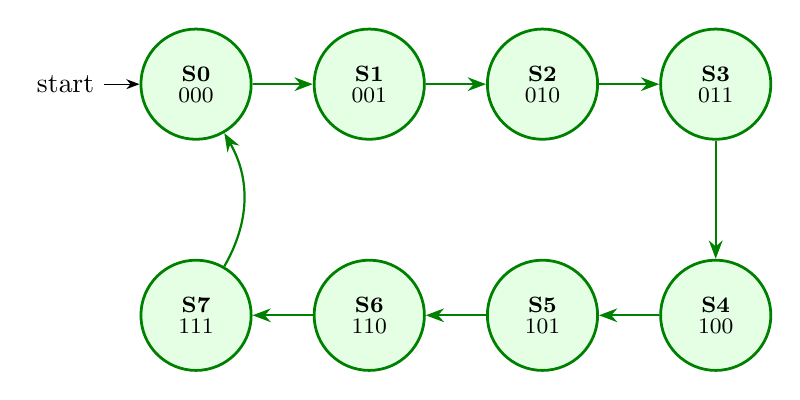
\begin{tikzpicture}[
        ->,
        >=Stealth,
        node distance=2.2cm,
        every state/.style={
            minimum size=1.4cm, 
            font=\footnotesize,
            fill=green!10,
            draw=green!50!black,
            line width=1pt,
            align=center
        },
        auto
    ]
        % States in a row for binary
        \node[state, initial] (S0) {\textbf{S0}\\[-2pt]000};
        \node[state, right of=S0] (S1) {\textbf{S1}\\[-2pt]001};
        \node[state, right of=S1] (S2) {\textbf{S2}\\[-2pt]010};
        \node[state, right of=S2] (S3) {\textbf{S3}\\[-2pt]011};
        \node[state, below=1.5cm of S3] (S4) {\textbf{S4}\\[-2pt]100};
        \node[state, left of=S4] (S5) {\textbf{S5}\\[-2pt]101};
        \node[state, left of=S5] (S6) {\textbf{S6}\\[-2pt]110};
        \node[state, left of=S6] (S7) {\textbf{S7}\\[-2pt]111};
        
        % Binary transitions - clean sequential arrows
        \draw[thick, green!50!black] (S0) -- (S1);
        \draw[thick, green!50!black] (S1) -- (S2);
        \draw[thick, green!50!black] (S2) -- (S3);
        \draw[thick, green!50!black] (S3) -- (S4);
        \draw[thick, green!50!black] (S4) -- (S5);
        \draw[thick, green!50!black] (S5) -- (S6);
        \draw[thick, green!50!black] (S6) -- (S7);
        \draw[thick, green!50!black] (S7) to[bend right=30] (S0);
    \end{tikzpicture}
    \caption{Binary Mode (m=0): Simple Sequential Counting 0$\rightarrow$1$\rightarrow$2$\rightarrow$3$\rightarrow$4$\rightarrow$5$\rightarrow$6$\rightarrow$7$\rightarrow$0}
\end{figure}

\textbf{Explanation:} In binary mode, we simply go to the next state in order. S0$\rightarrow$S1$\rightarrow$S2$\rightarrow$S3$\rightarrow$S4$\rightarrow$S5$\rightarrow$S6$\rightarrow$S7$\rightarrow$back to S0.

\subsection{FSM State Diagram - Gray Code Mode (m=1)}

Now let's see the \textbf{Gray code counting} path (notice the ``jumps''):

\begin{figure}[H]
    \centering
    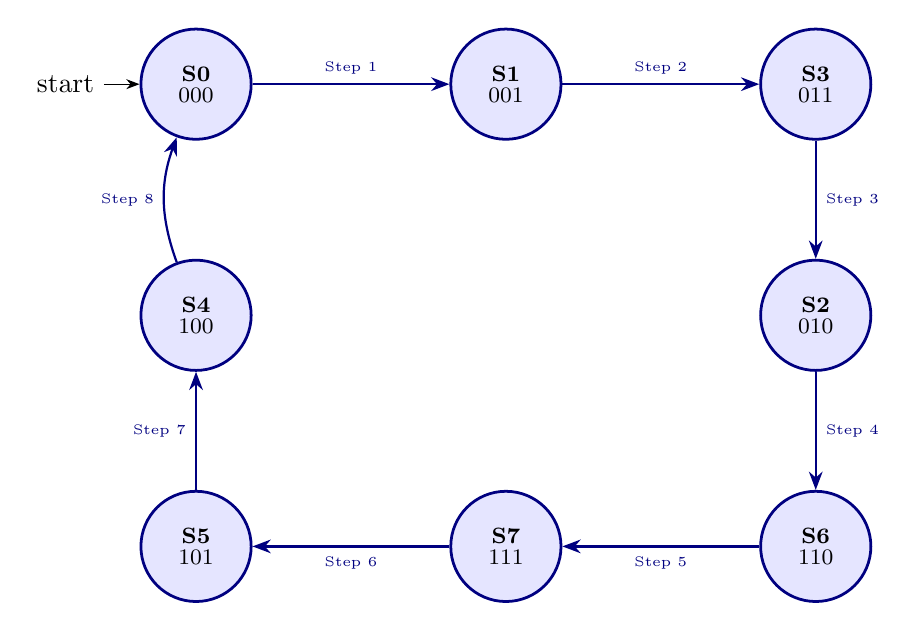
\begin{tikzpicture}[
        ->,
        >=Stealth,
        node distance=2.2cm,
        every state/.style={
            minimum size=1.4cm, 
            font=\footnotesize,
            fill=blue!10,
            draw=blue!50!black,
            line width=1pt,
            align=center
        },
        auto
    ]
        % States arranged for Gray code visibility
        \node[state, initial] (S0) {\textbf{S0}\\[-2pt]000};
        \node[state, right=2.5cm of S0] (S1) {\textbf{S1}\\[-2pt]001};
        \node[state, right=2.5cm of S1] (S3) {\textbf{S3}\\[-2pt]011};
        \node[state, below=1.5cm of S3] (S2) {\textbf{S2}\\[-2pt]010};
        \node[state, below=1.5cm of S2] (S6) {\textbf{S6}\\[-2pt]110};
        \node[state, left=2.5cm of S6] (S7) {\textbf{S7}\\[-2pt]111};
        \node[state, left=2.5cm of S7] (S5) {\textbf{S5}\\[-2pt]101};
        \node[state, above=1.5cm of S5] (S4) {\textbf{S4}\\[-2pt]100};
        
        % Gray code transitions with step numbers
        \draw[thick, blue!50!black] (S0) -- node[above] {\tiny Step 1} (S1);
        \draw[thick, blue!50!black] (S1) -- node[above] {\tiny Step 2} (S3);
        \draw[thick, blue!50!black] (S3) -- node[right] {\tiny Step 3} (S2);
        \draw[thick, blue!50!black] (S2) -- node[right] {\tiny Step 4} (S6);
        \draw[thick, blue!50!black] (S6) -- node[below] {\tiny Step 5} (S7);
        \draw[thick, blue!50!black] (S7) -- node[below] {\tiny Step 6} (S5);
        \draw[thick, blue!50!black] (S5) -- node[left] {\tiny Step 7} (S4);
        \draw[thick, blue!50!black] (S4) to[bend left=20] node[left] {\tiny Step 8} (S0);
    \end{tikzpicture}
    \caption{Gray Code Mode (m=1): Non-Sequential Path 0$\rightarrow$1$\rightarrow$3$\rightarrow$2$\rightarrow$6$\rightarrow$7$\rightarrow$5$\rightarrow$4$\rightarrow$0}
\end{figure}

\textbf{Explanation:} In Gray code mode, we DON'T go in order! We jump: S0$\rightarrow$S1$\rightarrow$S3$\rightarrow$S2$\rightarrow$S6$\rightarrow$S7$\rightarrow$S5$\rightarrow$S4$\rightarrow$back to S0. This ensures only one bit changes each step.

\subsection{Combined FSM State Diagram}

Now let's combine both modes into one diagram:

\begin{figure}[H]
    \centering
    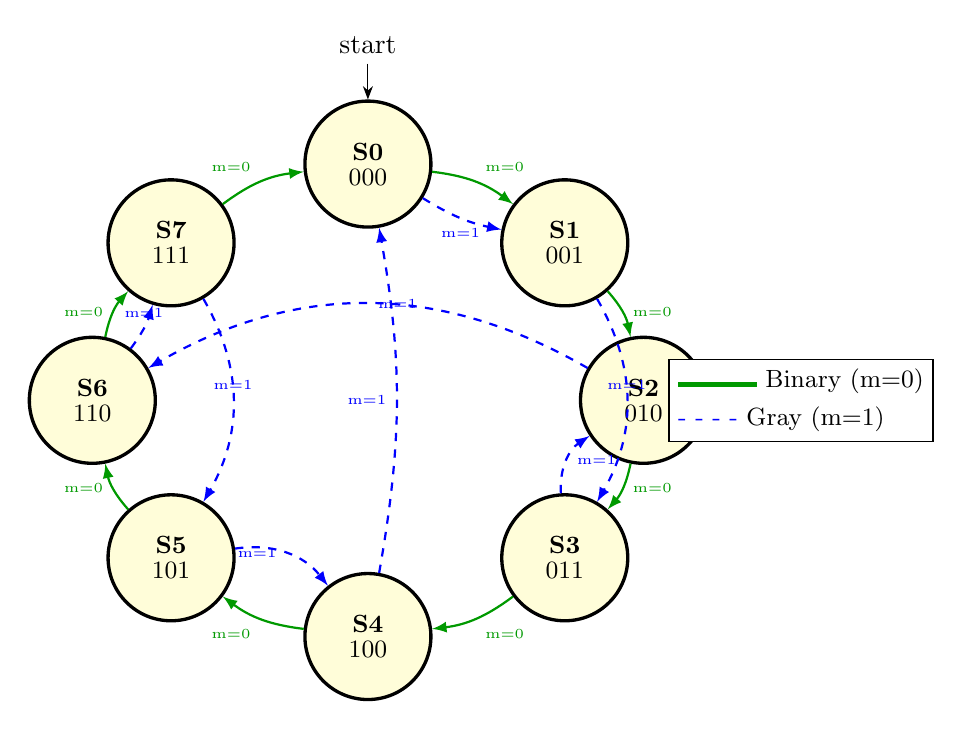
\begin{tikzpicture}[
        ->,
        >=Stealth,
        node distance=2.8cm,
        every state/.style={
            minimum size=1.6cm, 
            font=\small,
            fill=yellow!15,
            draw=black,
            line width=1.2pt,
            align=center
        },
        auto
    ]
        % States in octagon layout
        \node[state, initial above] (S0) at (0,3) {\textbf{S0}\\[-2pt]000};
        \node[state] (S1) at (2.5,2) {\textbf{S1}\\[-2pt]001};
        \node[state] (S2) at (3.5,0) {\textbf{S2}\\[-2pt]010};
        \node[state] (S3) at (2.5,-2) {\textbf{S3}\\[-2pt]011};
        \node[state] (S4) at (0,-3) {\textbf{S4}\\[-2pt]100};
        \node[state] (S5) at (-2.5,-2) {\textbf{S5}\\[-2pt]101};
        \node[state] (S6) at (-3.5,0) {\textbf{S6}\\[-2pt]110};
        \node[state] (S7) at (-2.5,2) {\textbf{S7}\\[-2pt]111};
        
        % Binary mode transitions (m=0) - GREEN solid arrows (outer ring)
        \draw[thick, green!60!black, ->, >=latex] (S0) to[bend left=15] node[above right, font=\tiny, green!60!black] {m=0} (S1);
        \draw[thick, green!60!black, ->, >=latex] (S1) to[bend left=15] node[right, font=\tiny, green!60!black] {m=0} (S2);
        \draw[thick, green!60!black, ->, >=latex] (S2) to[bend left=15] node[right, font=\tiny, green!60!black] {m=0} (S3);
        \draw[thick, green!60!black, ->, >=latex] (S3) to[bend left=15] node[below right, font=\tiny, green!60!black] {m=0} (S4);
        \draw[thick, green!60!black, ->, >=latex] (S4) to[bend left=15] node[below left, font=\tiny, green!60!black] {m=0} (S5);
        \draw[thick, green!60!black, ->, >=latex] (S5) to[bend left=15] node[left, font=\tiny, green!60!black] {m=0} (S6);
        \draw[thick, green!60!black, ->, >=latex] (S6) to[bend left=15] node[left, font=\tiny, green!60!black] {m=0} (S7);
        \draw[thick, green!60!black, ->, >=latex] (S7) to[bend left=15] node[above left, font=\tiny, green!60!black] {m=0} (S0);
        
        % Gray code transitions (m=1) - BLUE dashed arrows (crossing)
        \draw[thick, blue, dashed, ->, >=latex] (S0) to[bend right=10] node[below, font=\tiny, blue] {m=1} (S1);
        \draw[thick, blue, dashed, ->, >=latex] (S1) to[bend left=30] node[above, font=\tiny, blue] {m=1} (S3);
        \draw[thick, blue, dashed, ->, >=latex] (S3) to[bend left=30] node[right, font=\tiny, blue] {m=1} (S2);
        \draw[thick, blue, dashed, ->, >=latex] (S2) to[bend right=30] node[right, font=\tiny, blue] {m=1} (S6);
        \draw[thick, blue, dashed, ->, >=latex] (S6) to[bend right=10] node[above, font=\tiny, blue] {m=1} (S7);
        \draw[thick, blue, dashed, ->, >=latex] (S7) to[bend left=30] node[above, font=\tiny, blue] {m=1} (S5);
        \draw[thick, blue, dashed, ->, >=latex] (S5) to[bend left=30] node[left, font=\tiny, blue] {m=1} (S4);
        \draw[thick, blue, dashed, ->, >=latex] (S4) to[bend right=10] node[left, font=\tiny, blue] {m=1} (S0);
        
        % Legend
        \node[draw, fill=white, align=left, font=\small] at (5.5, 0) {
            \textcolor{green!60!black}{\rule{1cm}{2pt}} Binary (m=0)\\[3pt]
            \textcolor{blue}{- - - -} Gray (m=1)
        };
    \end{tikzpicture}
    \caption{Complete Multi-Mode Counter FSM: Green Solid = Binary, Blue Dashed = Gray Code}
\end{figure}

\subsection{Step-by-Step: How the FSM Works}

\subsubsection{Example 1: Binary Mode (m=0)}
\begin{enumerate}
    \item Start at \textbf{S0} (output = 000)
    \item Clock tick $\rightarrow$ Go to \textbf{S1} (output = 001)
    \item Clock tick $\rightarrow$ Go to \textbf{S2} (output = 010)
    \item Clock tick $\rightarrow$ Go to \textbf{S3} (output = 011)
    \item ... and so on in sequence
\end{enumerate}

\subsubsection{Example 2: Gray Mode (m=1)}
\begin{enumerate}
    \item Start at \textbf{S0} (output = 000)
    \item Clock tick $\rightarrow$ Go to \textbf{S1} (output = 001) - bit 0 changed
    \item Clock tick $\rightarrow$ \textbf{JUMP} to \textbf{S3} (output = 011) - bit 1 changed
    \item Clock tick $\rightarrow$ Go to \textbf{S2} (output = 010) - bit 0 changed
    \item Clock tick $\rightarrow$ \textbf{JUMP} to \textbf{S6} (output = 110) - bit 2 changed
    \item ... and so on following Gray code sequence
\end{enumerate}

\subsubsection{Example 3: Switching Modes Mid-Count}
\begin{enumerate}
    \item Currently at \textbf{S3} in Binary mode (output = 011)
    \item User switches mode to Gray (m=1)
    \item Clock tick $\rightarrow$ Go to \textbf{S2} (following Gray path from S3)
    \item The output is still determined by the state, not the mode!
\end{enumerate}

\subsection{State Transition Table}

\begin{table}[H]
    \centering
    \begin{tabular}{|c|c|c|c|c|}
        \hline
        \textbf{Current State} & \textbf{Output} & \textbf{m=0 (Binary)} & \textbf{m=1 (Gray)} \\
        \hline
        S0 & 000 & S1 & S1 \\
        S1 & 001 & S2 & S3 \\
        S2 & 010 & S3 & S6 \\
        S3 & 011 & S4 & S2 \\
        S4 & 100 & S5 & S0 \\
        S5 & 101 & S6 & S4 \\
        S6 & 110 & S7 & S7 \\
        S7 & 111 & S0 & S5 \\
        \hline
    \end{tabular}
    \caption{State Transition Table for Multi-Mode Counter}
\end{table}

\subsection{Gray Code Sequence - Detailed Explanation}

The Gray code sequence ensures only one bit changes between consecutive values. Let's trace through each transition:

\begin{table}[H]
    \centering
    \begin{tabular}{|c|c|c|c|c|l|}
        \hline
        \textbf{Step} & \textbf{State} & \textbf{Output} & \textbf{Bit 2} & \textbf{Bit 1} & \textbf{Bit 0} \\
        \hline
        1 & S0 & 000 & 0 & 0 & 0 \\
        2 & S1 & 001 & 0 & 0 & \textcolor{red}{\textbf{1}} $\leftarrow$ changed \\
        3 & S3 & 011 & 0 & \textcolor{red}{\textbf{1}} & 1 $\leftarrow$ changed \\
        4 & S2 & 010 & 0 & 1 & \textcolor{red}{\textbf{0}} $\leftarrow$ changed \\
        5 & S6 & 110 & \textcolor{red}{\textbf{1}} & 1 & 0 $\leftarrow$ changed \\
        6 & S7 & 111 & 1 & 1 & \textcolor{red}{\textbf{1}} $\leftarrow$ changed \\
        7 & S5 & 101 & 1 & \textcolor{red}{\textbf{0}} & 1 $\leftarrow$ changed \\
        8 & S4 & 100 & 1 & 0 & \textcolor{red}{\textbf{0}} $\leftarrow$ changed \\
        \hline
    \end{tabular}
    \caption{Gray Code Sequence - Only ONE bit changes per step (shown in red)}
\end{table}

\textbf{Why is this useful?}
\begin{itemize}
    \item In binary counting (0$\rightarrow$1$\rightarrow$2), when going from 001 to 010, \textbf{TWO bits} change simultaneously
    \item This can cause \textbf{glitches} in hardware because bits don't change at exactly the same moment
    \item Gray code avoids this by ensuring only \textbf{ONE bit} ever changes at a time
\end{itemize}

\subsection{VHDL Implementation}

\begin{lstlisting}[caption={multi\_mode\_counter.vhd}]
library ieee;
use ieee.std_logic_1164.all;

entity multi_mode_counter is
    port (
        clk   : in  std_logic;
        rst   : in  std_logic;
        m     : in  std_logic;  -- 0=Binary, 1=Gray
        count : out std_logic_vector(2 downto 0)
    );
end multi_mode_counter;

architecture bhv of multi_mode_counter is
    type state_type is (s0, s1, s2, s3, s4, s5, s6, s7);
    signal current_state, next_state : state_type;
begin

    ------------ Process 1: State Register ------------
    process(clk, rst)
    begin
        if rst = '1' then
            current_state <= s0;
        elsif rising_edge(clk) then
            current_state <= next_state;
        end if;
    end process;

    ------------ Process 2: Next State Logic ------------
    process(current_state, m)
    begin
        case current_state is
            when s0 =>
                if m = '0' then
                    next_state <= s1;  -- Binary: 0->1
                else
                    next_state <= s1;  -- Gray: 0->1
                end if;
            when s1 =>
                if m = '0' then
                    next_state <= s2;  -- Binary: 1->2
                else
                    next_state <= s3;  -- Gray: 1->3
                end if;
            when s2 =>
                if m = '0' then
                    next_state <= s3;  -- Binary: 2->3
                else
                    next_state <= s6;  -- Gray: 2->6
                end if;
            when s3 =>
                if m = '0' then
                    next_state <= s4;  -- Binary: 3->4
                else
                    next_state <= s2;  -- Gray: 3->2
                end if;
            when s4 =>
                if m = '0' then
                    next_state <= s5;  -- Binary: 4->5
                else
                    next_state <= s0;  -- Gray: 4->0 (wrap)
                end if;
            when s5 =>
                if m = '0' then
                    next_state <= s6;  -- Binary: 5->6
                else
                    next_state <= s4;  -- Gray: 5->4
                end if;
            when s6 =>
                if m = '0' then
                    next_state <= s7;  -- Binary: 6->7
                else
                    next_state <= s7;  -- Gray: 6->7
                end if;
            when s7 =>
                if m = '0' then
                    next_state <= s0;  -- Binary: 7->0 (wrap)
                else
                    next_state <= s5;  -- Gray: 7->5
                end if;
        end case;
    end process;

    ------------ Process 3: Output Logic (Moore) ------------
    process(current_state)
    begin
        case current_state is
            when s0 => count <= "000";
            when s1 => count <= "001";
            when s2 => count <= "010";
            when s3 => count <= "011";
            when s4 => count <= "100";
            when s5 => count <= "101";
            when s6 => count <= "110";
            when s7 => count <= "111";
        end case;
    end process;

end bhv;
\end{lstlisting}

\subsection{Testbench}

\begin{lstlisting}[caption={multi\_mode\_counter\_tb.vhd}]
library ieee;
use ieee.std_logic_1164.all;

entity multi_mode_counter_tb is
end multi_mode_counter_tb;

architecture sim of multi_mode_counter_tb is
    signal clk   : std_logic := '0';
    signal rst   : std_logic := '0';
    signal m     : std_logic := '0';
    signal count : std_logic_vector(2 downto 0);
    
    constant CLK_PERIOD : time := 10 ns;
begin

    -- Instantiate DUT
    DUT: entity work.multi_mode_counter
        port map (
            clk   => clk,
            rst   => rst,
            m     => m,
            count => count
        );

    -- Clock generation
    clk <= not clk after CLK_PERIOD/2;

    -- Stimulus process
    process
    begin
        -- Reset
        rst <= '1';
        wait for 20 ns;
        rst <= '0';
        
        -- Test Binary mode (m=0)
        m <= '0';
        wait for 100 ns;  -- Count through 0-7
        
        -- Test Gray mode (m=1)
        m <= '1';
        rst <= '1';
        wait for 10 ns;
        rst <= '0';
        wait for 100 ns;  -- Count through Gray sequence
        
        -- End simulation
        wait;
    end process;

end sim;
\end{lstlisting}

\newpage
% ============================================================
\section{In-Lab Task 2: Vending Machine Design (Moore FSM)}
% ============================================================

\subsection{Understanding the Problem}

We need to design a \textbf{soft-drink dispensing machine} that:
\begin{enumerate}
    \item Accepts coins and keeps track of total credit
    \item Allows user to select a drink
    \item Dispenses the drink if enough credit is available
    \item Returns the correct change
\end{enumerate}

\subsection{Machine Specifications}

\subsubsection{Accepted Coins}
The machine accepts 4 types of coins:

\begin{table}[H]
    \centering
    \begin{tabular}{|c|c|c|}
        \hline
        \textbf{Coin Input} & \textbf{Value} & \textbf{Signal Name} \\
        \hline
        Rs. 1 coin & 1 & \texttt{coin\_1} \\
        Rs. 2 coin & 2 & \texttt{coin\_2} \\
        Rs. 4 coin & 4 & \texttt{coin\_4} \\
        Rs. 8 coin & 8 & \texttt{coin\_8} \\
        \hline
    \end{tabular}
    \caption{Accepted Coins and Signal Names}
\end{table}

\subsubsection{Available Drinks}
\begin{table}[H]
    \centering
    \begin{tabular}{|c|c|c|c|}
        \hline
        \textbf{Drink} & \textbf{Price (Rs.)} & \textbf{Selection Signal} & \textbf{Dispense Signal} \\
        \hline
        Rango & 3 & \texttt{sel\_rango} & \texttt{disp\_rango} \\
        Next & 4 & \texttt{sel\_next} & \texttt{disp\_next} \\
        Fizup & 5 & \texttt{sel\_fizup} & \texttt{disp\_fizup} \\
        \hline
    \end{tabular}
    \caption{Drink Options with Prices and Signals}
\end{table}

\subsubsection{Machine Rules}
\begin{enumerate}
    \item \textbf{Sufficient credit required:} Customer must deposit enough money before buying
    \item \textbf{Single coin at a time:} Machine ignores multiple coins inserted simultaneously
    \item \textbf{Single selection at a time:} Multiple drink selections are ignored
    \item \textbf{Maximum credit = Rs. 15:} Additional coins beyond this are returned immediately
    \item \textbf{Coin return:} Pressing ENTER without selection returns all credit as change
\end{enumerate}

\subsection{System Block Diagram}

\begin{figure}[H]
    \centering
    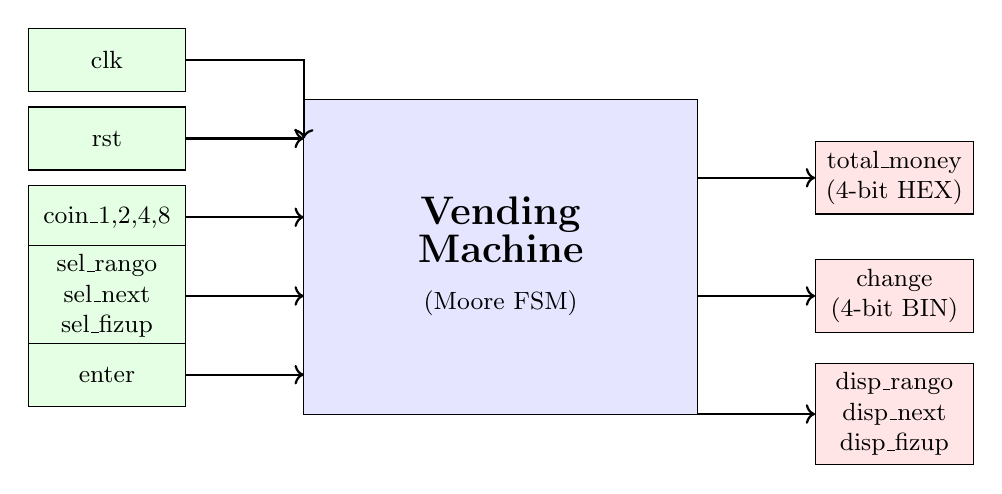
\begin{tikzpicture}[
        block/.style={rectangle, draw, fill=blue!10, minimum width=3cm, minimum height=1.5cm, align=center},
        input/.style={rectangle, draw, fill=green!10, minimum width=2cm, minimum height=0.8cm, align=center, font=\small},
        output/.style={rectangle, draw, fill=red!10, minimum width=2cm, minimum height=0.8cm, align=center, font=\small}
    ]
        % Main block
        \node[block, minimum width=5cm, minimum height=4cm] (vm) at (0,0) {\Large\textbf{Vending}\\\Large\textbf{Machine}\\[5pt]\small (Moore FSM)};
        
        % Inputs on left
        \node[input] (clk) at (-5, 2.5) {clk};
        \node[input] (rst) at (-5, 1.5) {rst};
        \node[input] (coins) at (-5, 0.5) {coin\_1,2,4,8};
        \node[input] (drinks) at (-5, -0.5) {sel\_rango\\sel\_next\\sel\_fizup};
        \node[input] (enter) at (-5, -1.5) {enter};
        
        % Outputs on right
        \node[output] (total) at (5, 1) {total\_money\\(4-bit HEX)};
        \node[output] (change) at (5, -0.5) {change\\(4-bit BIN)};
        \node[output] (disp) at (5, -2) {disp\_rango\\disp\_next\\disp\_fizup};
        
        % Arrows
        \draw[->, thick] (clk) -- (-2.5, 2.5) -- (-2.5, 1.5);
        \draw[->, thick] (rst) -- (-2.5, 1.5);
        \draw[->, thick] (coins) -- (-2.5, 0.5);
        \draw[->, thick] (drinks) -- (-2.5, -0.5);
        \draw[->, thick] (enter) -- (-2.5, -1.5);
        
        \draw[->, thick] (2.5, 1) -- (total);
        \draw[->, thick] (2.5, -0.5) -- (change);
        \draw[->, thick] (2.5, -2) -- (disp);
    \end{tikzpicture}
    \caption{Vending Machine Block Diagram - Inputs and Outputs}
\end{figure}

\subsection{Why Moore Machine?}

\begin{table}[H]
    \centering
    \begin{tabular}{|p{4cm}|p{5cm}|p{5cm}|}
        \hline
        \textbf{Feature} & \textbf{Moore (We Use This)} & \textbf{Mealy (Alternative)} \\
        \hline
        Output depends on & \textbf{State ONLY} & State + Input \\
        \hline
        When output changes & On clock edge only & Immediately with input \\
        \hline
        Stability & Very stable & Can have glitches \\
        \hline
        For vending machine & Safe - drink dispenses only after state is confirmed & Risky - noisy input could cause partial dispense \\
        \hline
    \end{tabular}
    \caption{Why Moore is Better for Vending Machine}
\end{table}

\textbf{Key Point:} In a real vending machine, we don't want the drink dispenser to activate based on a noisy button press. Moore ensures the output is stable and only changes when the state officially changes on a clock edge.

\subsection{State Design - The Heart of the FSM}

\subsubsection{What Should Each State Represent?}

Each state represents the \textbf{current credit amount} in the machine:

\begin{table}[H]
    \centering
    \begin{tabular}{|c|c|l|l|}
        \hline
        \textbf{State} & \textbf{Credit} & \textbf{Can Buy} & \textbf{Output (total\_money)} \\
        \hline
        S0 & Rs. 0 & Nothing & 0000 (0x0) \\
        S1 & Rs. 1 & Nothing & 0001 (0x1) \\
        S2 & Rs. 2 & Nothing & 0010 (0x2) \\
        \rowcolor{green!20} S3 & Rs. 3 & \textbf{Rango} & 0011 (0x3) \\
        \rowcolor{green!20} S4 & Rs. 4 & \textbf{Rango, Next} & 0100 (0x4) \\
        \rowcolor{green!20} S5 & Rs. 5 & \textbf{All drinks} & 0101 (0x5) \\
        \rowcolor{green!20} S6 & Rs. 6 & \textbf{All drinks} & 0110 (0x6) \\
        \rowcolor{green!20} S7 & Rs. 7 & \textbf{All drinks} & 0111 (0x7) \\
        \rowcolor{green!20} S8 & Rs. 8 & \textbf{All drinks} & 1000 (0x8) \\
        ... & ... & ... & ... \\
        \rowcolor{green!20} S15 & Rs. 15 & \textbf{All drinks (MAX)} & 1111 (0xF) \\
        \hline
    \end{tabular}
    \caption{All 16 States and What Can Be Purchased (Green = Can Buy Something)}
\end{table}

\subsection{FSM State Diagram - Adding Coins}

\begin{figure}[H]
    \centering
    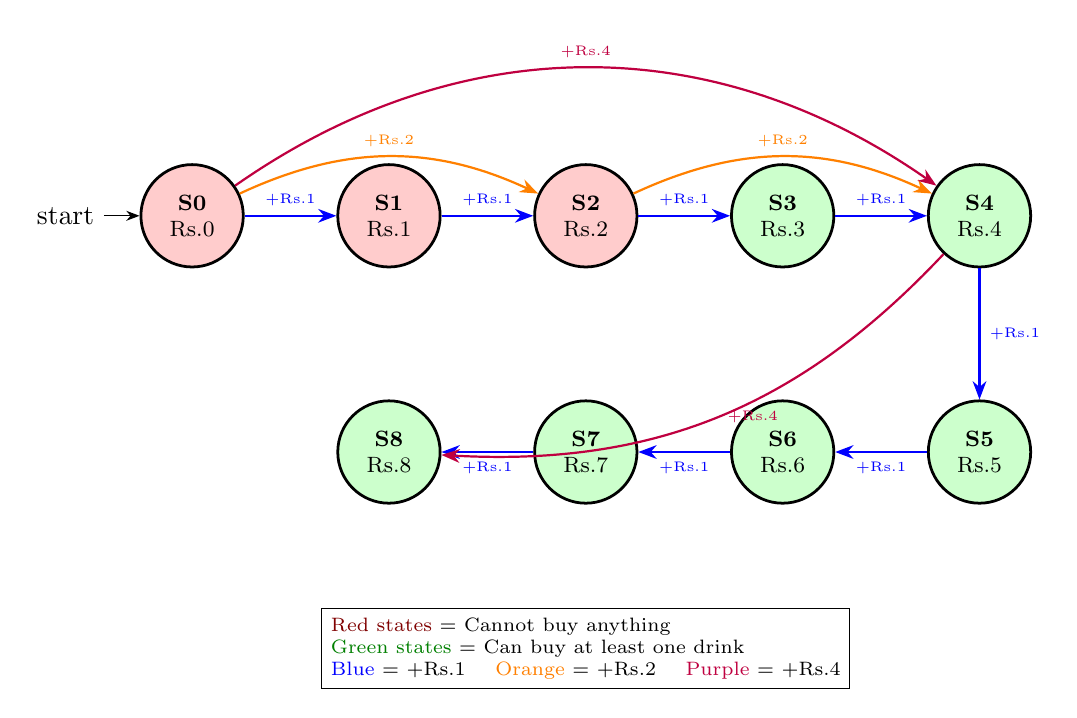
\begin{tikzpicture}[
        ->,
        >=Stealth,
        node distance=2cm,
        every state/.style={
            minimum size=1.3cm, 
            font=\footnotesize,
            fill=yellow!20,
            draw=black,
            line width=1pt,
            align=center
        },
        auto
    ]
        % States - first row
        \node[state, initial, fill=red!20] (S0) at (0,0) {\textbf{S0}\\Rs.0};
        \node[state, fill=red!20] (S1) at (2.5,0) {\textbf{S1}\\Rs.1};
        \node[state, fill=red!20] (S2) at (5,0) {\textbf{S2}\\Rs.2};
        \node[state, fill=green!20] (S3) at (7.5,0) {\textbf{S3}\\Rs.3};
        \node[state, fill=green!20] (S4) at (10,0) {\textbf{S4}\\Rs.4};
        
        % States - second row
        \node[state, fill=green!20] (S5) at (10,-3) {\textbf{S5}\\Rs.5};
        \node[state, fill=green!20] (S6) at (7.5,-3) {\textbf{S6}\\Rs.6};
        \node[state, fill=green!20] (S7) at (5,-3) {\textbf{S7}\\Rs.7};
        \node[state, fill=green!20] (S8) at (2.5,-3) {\textbf{S8}\\Rs.8};
        
        % +1 transitions (top row)
        \draw[thick, blue] (S0) -- node[above] {\tiny +Rs.1} (S1);
        \draw[thick, blue] (S1) -- node[above] {\tiny +Rs.1} (S2);
        \draw[thick, blue] (S2) -- node[above] {\tiny +Rs.1} (S3);
        \draw[thick, blue] (S3) -- node[above] {\tiny +Rs.1} (S4);
        \draw[thick, blue] (S4) -- node[right] {\tiny +Rs.1} (S5);
        
        % +1 transitions (bottom row)
        \draw[thick, blue] (S5) -- node[below] {\tiny +Rs.1} (S6);
        \draw[thick, blue] (S6) -- node[below] {\tiny +Rs.1} (S7);
        \draw[thick, blue] (S7) -- node[below] {\tiny +Rs.1} (S8);
        
        % +2 transitions (jumping)
        \draw[thick, orange, bend left=25] (S0) to node[above] {\tiny +Rs.2} (S2);
        \draw[thick, orange, bend left=25] (S2) to node[above] {\tiny +Rs.2} (S4);
        
        % +4 transitions (bigger jumps)
        \draw[thick, purple, bend left=35] (S0) to node[above] {\tiny +Rs.4} (S4);
        \draw[thick, purple, bend left=25] (S4) to node[right] {\tiny +Rs.4} (S8);
        
        % Legend
        \node[draw, fill=white, align=left, font=\scriptsize] at (5, -5.5) {
            \textcolor{red!50!black}{Red states} = Cannot buy anything\\
            \textcolor{green!50!black}{Green states} = Can buy at least one drink\\
            \textcolor{blue}{Blue} = +Rs.1 \quad \textcolor{orange}{Orange} = +Rs.2 \quad \textcolor{purple}{Purple} = +Rs.4
        };
    \end{tikzpicture}
    \caption{FSM Coin Addition - How Credit Increases (Partial View)}
\end{figure}

\subsection{FSM State Diagram - Dispensing Drinks}

When ENTER is pressed with a drink selected, the machine dispenses and returns to a lower state:

\begin{figure}[H]
    \centering
    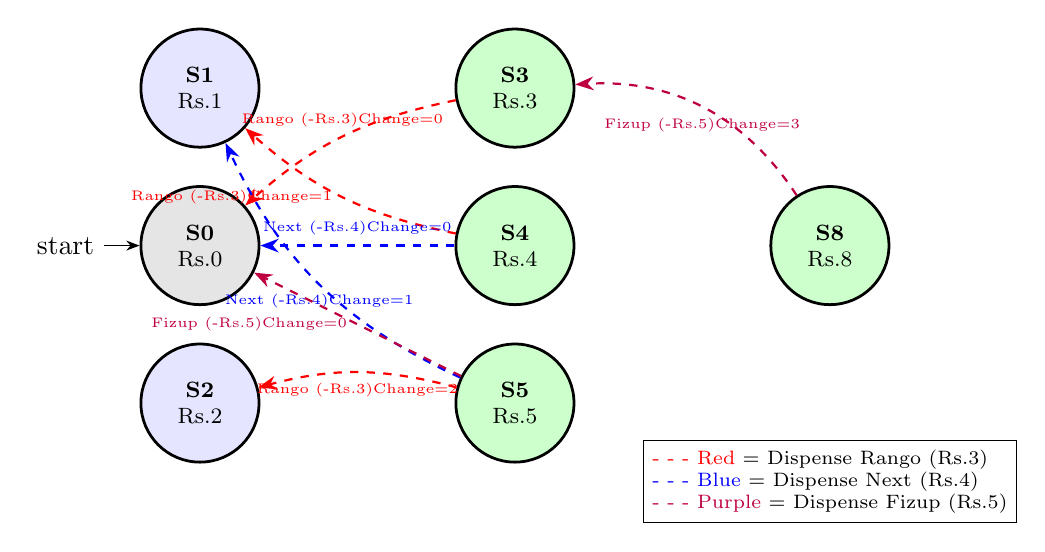
\begin{tikzpicture}[
        ->,
        >=Stealth,
        node distance=2.2cm,
        every state/.style={
            minimum size=1.5cm, 
            font=\footnotesize,
            fill=yellow!20,
            draw=black,
            line width=1pt,
            align=center
        },
        auto
    ]
        % Key states
        \node[state, initial, fill=gray!20] (S0) at (0,0) {\textbf{S0}\\Rs.0};
        \node[state, fill=green!20] (S3) at (4,2) {\textbf{S3}\\Rs.3};
        \node[state, fill=green!20] (S4) at (4,0) {\textbf{S4}\\Rs.4};
        \node[state, fill=green!20] (S5) at (4,-2) {\textbf{S5}\\Rs.5};
        \node[state, fill=green!20] (S8) at (8,0) {\textbf{S8}\\Rs.8};
        
        % Intermediate states for change
        \node[state, fill=blue!10] (S1) at (0,2) {\textbf{S1}\\Rs.1};
        \node[state, fill=blue!10] (S2) at (0,-2) {\textbf{S2}\\Rs.2};
        
        % Dispense Rango (Rs.3)
        \draw[thick, red, dashed] (S3) to[bend right=15] node[above, font=\tiny] {Rango (-Rs.3)\\Change=0} (S0);
        \draw[thick, red, dashed] (S4) to[bend left=15] node[left, font=\tiny] {Rango (-Rs.3)\\Change=1} (S1);
        \draw[thick, red, dashed] (S5) to[bend right=15] node[below, font=\tiny] {Rango (-Rs.3)\\Change=2} (S2);
        
        % Dispense Next (Rs.4)
        \draw[thick, blue, dashed] (S4) to node[above, font=\tiny] {Next (-Rs.4)\\Change=0} (S0);
        \draw[thick, blue, dashed] (S5) to[bend left=20] node[below, font=\tiny] {Next (-Rs.4)\\Change=1} (S1);
        
        % Dispense Fizup (Rs.5)
        \draw[thick, purple, dashed] (S5) to node[left, font=\tiny] {Fizup (-Rs.5)\\Change=0} (S0);
        \draw[thick, purple, dashed] (S8) to[bend right=30] node[below, font=\tiny] {Fizup (-Rs.5)\\Change=3} (S3);
        
        % Legend
        \node[draw, fill=white, align=left, font=\scriptsize] at (8, -3) {
            \textcolor{red}{- - - Red} = Dispense Rango (Rs.3)\\
            \textcolor{blue}{- - - Blue} = Dispense Next (Rs.4)\\
            \textcolor{purple}{- - - Purple} = Dispense Fizup (Rs.5)
        };
    \end{tikzpicture}
    \caption{FSM Drink Dispensing - State Transitions with Change Calculation}
\end{figure}

\subsection{Step-by-Step Example Scenarios}

\subsubsection{Scenario 1: Buy Rango with Exact Change}
\begin{enumerate}
    \item \textbf{Start:} Machine in S0 (Rs. 0 credit)
    \item \textbf{Insert Rs. 2 coin:} Machine transitions to S2 (Rs. 2 credit)
    \item \textbf{Insert Rs. 1 coin:} Machine transitions to S3 (Rs. 3 credit)
    \item \textbf{Select Rango + Press ENTER:}
    \begin{itemize}
        \item Credit (3) $\geq$ Rango price (3) $\checkmark$
        \item Dispense Rango: \texttt{disp\_rango = 1}
        \item Change = 3 - 3 = 0: \texttt{change = 0000}
        \item Transition to S0
    \end{itemize}
\end{enumerate}

\subsubsection{Scenario 2: Buy Next with Extra Money}
\begin{enumerate}
    \item \textbf{Start:} Machine in S0 (Rs. 0 credit)
    \item \textbf{Insert Rs. 8 coin:} Machine transitions to S8 (Rs. 8 credit)
    \item \textbf{Select Next + Press ENTER:}
    \begin{itemize}
        \item Credit (8) $\geq$ Next price (4) $\checkmark$
        \item Dispense Next: \texttt{disp\_next = 1}
        \item Change = 8 - 4 = 4: \texttt{change = 0100}
        \item Transition to S4 (remaining credit)
    \end{itemize}
    \item \textbf{Note:} User still has Rs. 4 credit! Can buy another drink or press ENTER to get change.
\end{enumerate}

\subsubsection{Scenario 3: Insufficient Funds}
\begin{enumerate}
    \item \textbf{Start:} Machine in S0
    \item \textbf{Insert Rs. 2 coin:} Machine transitions to S2 (Rs. 2 credit)
    \item \textbf{Select Fizup (Rs. 5) + Press ENTER:}
    \begin{itemize}
        \item Credit (2) $<$ Fizup price (5) $\times$
        \item \textbf{Nothing dispensed!}
        \item Machine stays in S2, waiting for more coins
    \end{itemize}
\end{enumerate}

\subsubsection{Scenario 4: Return Money Without Purchase}
\begin{enumerate}
    \item \textbf{Start:} Machine in S0
    \item \textbf{Insert Rs. 4 coin:} Machine transitions to S4
    \item \textbf{Insert Rs. 2 coin:} Machine transitions to S6 (Rs. 6 credit)
    \item \textbf{Press ENTER without selecting drink:}
    \begin{itemize}
        \item No drink selected
        \item Return all credit as change: \texttt{change = 0110} (6 in binary)
        \item Transition to S0
    \end{itemize}
\end{enumerate}

\subsection{Complete State Transition Table}

\begin{table}[H]
    \centering
    \footnotesize
    \begin{tabular}{|c|c|c|c|c|c|c|c|c|}
        \hline
        \textbf{Current} & \textbf{+Rs.1} & \textbf{+Rs.2} & \textbf{+Rs.4} & \textbf{+Rs.8} & \textbf{Rango} & \textbf{Next} & \textbf{Fizup} & \textbf{Output} \\
        \textbf{State} & & & & & \textbf{(-Rs.3)} & \textbf{(-Rs.4)} & \textbf{(-Rs.5)} & \\
        \hline
        S0 (Rs.0) & S1 & S2 & S4 & S8 & -- & -- & -- & 0000 \\
        S1 (Rs.1) & S2 & S3 & S5 & S9 & -- & -- & -- & 0001 \\
        S2 (Rs.2) & S3 & S4 & S6 & S10 & -- & -- & -- & 0010 \\
        S3 (Rs.3) & S4 & S5 & S7 & S11 & S0 & -- & -- & 0011 \\
        S4 (Rs.4) & S5 & S6 & S8 & S12 & S1 & S0 & -- & 0100 \\
        S5 (Rs.5) & S6 & S7 & S9 & S13 & S2 & S1 & S0 & 0101 \\
        S6 (Rs.6) & S7 & S8 & S10 & S14 & S3 & S2 & S1 & 0110 \\
        S7 (Rs.7) & S8 & S9 & S11 & S15 & S4 & S3 & S2 & 0111 \\
        S8 (Rs.8) & S9 & S10 & S12 & S15* & S5 & S4 & S3 & 1000 \\
        ... & ... & ... & ... & ... & ... & ... & ... & ... \\
        S15 (Rs.15) & S15* & S15* & S15* & S15* & S12 & S11 & S10 & 1111 \\
        \hline
    \end{tabular}
    \caption{State Transition Table (* = excess coins returned, -- = insufficient funds)}
\end{table}

\subsection{Change Calculation Formula}

\begin{equation}
\text{Change} = \text{Current Credit} - \text{Drink Price}
\end{equation}

\begin{table}[H]
    \centering
    \begin{tabular}{|c|c|c|c|c|}
        \hline
        \textbf{If Credit =} & \textbf{Buy Rango (Rs.3)} & \textbf{Buy Next (Rs.4)} & \textbf{Buy Fizup (Rs.5)} \\
        \hline
        Rs. 3 & Change = 0 & Cannot buy & Cannot buy \\
        Rs. 4 & Change = 1 & Change = 0 & Cannot buy \\
        Rs. 5 & Change = 2 & Change = 1 & Change = 0 \\
        Rs. 6 & Change = 3 & Change = 2 & Change = 1 \\
        Rs. 7 & Change = 4 & Change = 3 & Change = 2 \\
        Rs. 8 & Change = 5 & Change = 4 & Change = 3 \\
        \hline
    \end{tabular}
    \caption{Change Calculation Examples}
\end{table}

\subsection{Three-Process FSM Architecture}

The VHDL code follows the standard \textbf{three-process} Moore FSM pattern:

\begin{figure}[H]
    \centering
    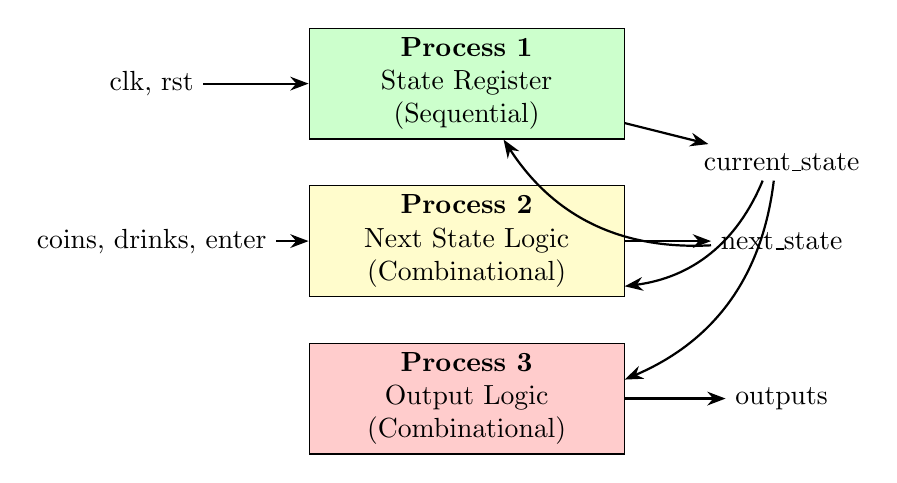
\begin{tikzpicture}[
        block/.style={rectangle, draw, fill=blue!10, minimum width=4cm, minimum height=1.2cm, align=center},
        arrow/.style={->, thick, >=Stealth}
    ]
        % Blocks
        \node[block, fill=green!20] (p1) at (0, 2) {\textbf{Process 1}\\State Register\\(Sequential)};
        \node[block, fill=yellow!20] (p2) at (0, 0) {\textbf{Process 2}\\Next State Logic\\(Combinational)};
        \node[block, fill=red!20] (p3) at (0, -2) {\textbf{Process 3}\\Output Logic\\(Combinational)};
        
        % Signals
        \node (clk) at (-4, 2) {clk, rst};
        \node (inputs) at (-4, 0) {coins, drinks, enter};
        \node (cs) at (4, 1) {current\_state};
        \node (ns) at (4, 0) {next\_state};
        \node (out) at (4, -2) {outputs};
        
        % Arrows
        \draw[arrow] (clk) -- (p1);
        \draw[arrow] (inputs) -- (p2);
        \draw[arrow] (p1) -- (cs);
        \draw[arrow] (cs) to[bend left=30] (p2);
        \draw[arrow] (cs) to[bend left=30] (p3);
        \draw[arrow] (p2) -- (ns);
        \draw[arrow] (ns) to[bend left=30] (p1);
        \draw[arrow] (p3) -- (out);
    \end{tikzpicture}
    \caption{Three-Process FSM Architecture}
\end{figure}

\subsection{VHDL Implementation}

\begin{lstlisting}[caption={vending\_machine.vhd}]
library ieee;
use ieee.std_logic_1164.all;
use ieee.numeric_std.all;

entity vending_machine is
    port (
        clk         : in  std_logic;
        rst         : in  std_logic;
        -- Coin inputs (active high, only one at a time)
        coin_1      : in  std_logic;  -- Rs. 1
        coin_2      : in  std_logic;  -- Rs. 2
        coin_4      : in  std_logic;  -- Rs. 4
        coin_8      : in  std_logic;  -- Rs. 8
        -- Drink selection (active high, only one at a time)
        sel_rango   : in  std_logic;  -- Rs. 3
        sel_next    : in  std_logic;  -- Rs. 4
        sel_fizup   : in  std_logic;  -- Rs. 5
        -- Control
        enter       : in  std_logic;
        -- Outputs
        total_money : out std_logic_vector(3 downto 0);  -- HEX
        change      : out std_logic_vector(3 downto 0);  -- Binary
        disp_rango  : out std_logic;
        disp_next   : out std_logic;
        disp_fizup  : out std_logic
    );
end vending_machine;

architecture bhv of vending_machine is
    -- States represent credit amount (0 to 15)
    type state_type is (s0, s1, s2, s3, s4, s5, s6, s7, 
                        s8, s9, s10, s11, s12, s13, s14, s15);
    signal current_state, next_state : state_type;
    
    -- Internal signals
    signal credit : integer range 0 to 15;
    signal coin_value : integer range 0 to 8;
    signal drink_price : integer range 0 to 5;
    signal change_amount : integer range 0 to 15;
    
begin

    ------------ Coin Value Decoder ------------
    coin_value <= 1 when coin_1 = '1' else
                  2 when coin_2 = '1' else
                  4 when coin_4 = '1' else
                  8 when coin_8 = '1' else
                  0;

    ------------ Drink Price Decoder ------------
    drink_price <= 3 when sel_rango = '1' else
                   4 when sel_next = '1' else
                   5 when sel_fizup = '1' else
                   0;

    ------------ Process 1: State Register ------------
    process(clk, rst)
    begin
        if rst = '1' then
            current_state <= s0;
        elsif rising_edge(clk) then
            current_state <= next_state;
        end if;
    end process;

    ------------ Process 2: Next State Logic ------------
    process(current_state, coin_value, drink_price, enter)
        variable new_credit : integer range 0 to 23;
    begin
        next_state <= current_state;  -- Default: stay
        
        -- State to credit mapping
        case current_state is
            when s0  => credit <= 0;
            when s1  => credit <= 1;
            when s2  => credit <= 2;
            when s3  => credit <= 3;
            when s4  => credit <= 4;
            when s5  => credit <= 5;
            when s6  => credit <= 6;
            when s7  => credit <= 7;
            when s8  => credit <= 8;
            when s9  => credit <= 9;
            when s10 => credit <= 10;
            when s11 => credit <= 11;
            when s12 => credit <= 12;
            when s13 => credit <= 13;
            when s14 => credit <= 14;
            when s15 => credit <= 15;
        end case;
        
        -- Add coin (if not at max)
        if coin_value > 0 and enter = '0' then
            new_credit := credit + coin_value;
            if new_credit > 15 then
                new_credit := 15;  -- Cap at max, return excess
            end if;
            -- Transition to new state
            case new_credit is
                when 0  => next_state <= s0;
                when 1  => next_state <= s1;
                when 2  => next_state <= s2;
                when 3  => next_state <= s3;
                when 4  => next_state <= s4;
                when 5  => next_state <= s5;
                when 6  => next_state <= s6;
                when 7  => next_state <= s7;
                when 8  => next_state <= s8;
                when 9  => next_state <= s9;
                when 10 => next_state <= s10;
                when 11 => next_state <= s11;
                when 12 => next_state <= s12;
                when 13 => next_state <= s13;
                when 14 => next_state <= s14;
                when 15 => next_state <= s15;
                when others => next_state <= s15;
            end case;
        end if;
        
        -- Dispense drink (when ENTER pressed)
        if enter = '1' then
            if drink_price > 0 and credit >= drink_price then
                -- Calculate remaining credit
                new_credit := credit - drink_price;
                case new_credit is
                    when 0  => next_state <= s0;
                    when 1  => next_state <= s1;
                    when 2  => next_state <= s2;
                    when 3  => next_state <= s3;
                    when 4  => next_state <= s4;
                    when 5  => next_state <= s5;
                    when 6  => next_state <= s6;
                    when 7  => next_state <= s7;
                    when 8  => next_state <= s8;
                    when 9  => next_state <= s9;
                    when 10 => next_state <= s10;
                    when others => next_state <= s0;
                end case;
            elsif drink_price = 0 then
                -- No drink selected, return all money
                next_state <= s0;
            end if;
        end if;
    end process;

    ------------ Process 3: Output Logic (Moore) ------------
    process(current_state, enter, drink_price, credit)
    begin
        -- Default outputs
        disp_rango <= '0';
        disp_next  <= '0';
        disp_fizup <= '0';
        change     <= "0000";
        
        -- Total money display (Moore output - depends on state)
        case current_state is
            when s0  => total_money <= "0000";
            when s1  => total_money <= "0001";
            when s2  => total_money <= "0010";
            when s3  => total_money <= "0011";
            when s4  => total_money <= "0100";
            when s5  => total_money <= "0101";
            when s6  => total_money <= "0110";
            when s7  => total_money <= "0111";
            when s8  => total_money <= "1000";
            when s9  => total_money <= "1001";
            when s10 => total_money <= "1010";
            when s11 => total_money <= "1011";
            when s12 => total_money <= "1100";
            when s13 => total_money <= "1101";
            when s14 => total_money <= "1110";
            when s15 => total_money <= "1111";
        end case;
        
        -- Dispense and change (when ENTER is pressed)
        if enter = '1' then
            if credit >= 3 and sel_rango = '1' then
                disp_rango <= '1';
                change <= std_logic_vector(to_unsigned(credit - 3, 4));
            elsif credit >= 4 and sel_next = '1' then
                disp_next <= '1';
                change <= std_logic_vector(to_unsigned(credit - 4, 4));
            elsif credit >= 5 and sel_fizup = '1' then
                disp_fizup <= '1';
                change <= std_logic_vector(to_unsigned(credit - 5, 4));
            else
                -- Return all money as change
                change <= std_logic_vector(to_unsigned(credit, 4));
            end if;
        end if;
    end process;

end bhv;
\end{lstlisting}

\newpage
\subsection{Testbench}

\begin{lstlisting}[caption={vending\_machine\_tb.vhd}]
library ieee;
use ieee.std_logic_1164.all;
use ieee.numeric_std.all;

entity vending_machine_tb is
end vending_machine_tb;

architecture sim of vending_machine_tb is
    signal clk         : std_logic := '0';
    signal rst         : std_logic := '0';
    signal coin_1      : std_logic := '0';
    signal coin_2      : std_logic := '0';
    signal coin_4      : std_logic := '0';
    signal coin_8      : std_logic := '0';
    signal sel_rango   : std_logic := '0';
    signal sel_next    : std_logic := '0';
    signal sel_fizup   : std_logic := '0';
    signal enter       : std_logic := '0';
    signal total_money : std_logic_vector(3 downto 0);
    signal change      : std_logic_vector(3 downto 0);
    signal disp_rango  : std_logic;
    signal disp_next   : std_logic;
    signal disp_fizup  : std_logic;
    
    constant CLK_PERIOD : time := 10 ns;
begin

    -- Instantiate DUT
    DUT: entity work.vending_machine
        port map (
            clk         => clk,
            rst         => rst,
            coin_1      => coin_1,
            coin_2      => coin_2,
            coin_4      => coin_4,
            coin_8      => coin_8,
            sel_rango   => sel_rango,
            sel_next    => sel_next,
            sel_fizup   => sel_fizup,
            enter       => enter,
            total_money => total_money,
            change      => change,
            disp_rango  => disp_rango,
            disp_next   => disp_next,
            disp_fizup  => disp_fizup
        );

    -- Clock generation
    clk <= not clk after CLK_PERIOD/2;

    -- Stimulus process
    process
    begin
        -- Reset
        rst <= '1';
        wait for 20 ns;
        rst <= '0';
        wait for 10 ns;
        
        -- Test Case 1: Buy Rango (Rs.3) with Rs.4
        -- Insert Rs.4 coin
        coin_4 <= '1';
        wait for CLK_PERIOD;
        coin_4 <= '0';
        wait for CLK_PERIOD;
        
        -- Select Rango and press Enter
        sel_rango <= '1';
        enter <= '1';
        wait for CLK_PERIOD;
        sel_rango <= '0';
        enter <= '0';
        wait for 20 ns;
        
        -- Test Case 2: Buy Fizup (Rs.5) with Rs.8
        rst <= '1';
        wait for 10 ns;
        rst <= '0';
        wait for 10 ns;
        
        -- Insert Rs.8 coin
        coin_8 <= '1';
        wait for CLK_PERIOD;
        coin_8 <= '0';
        wait for CLK_PERIOD;
        
        -- Select Fizup and press Enter
        sel_fizup <= '1';
        enter <= '1';
        wait for CLK_PERIOD;
        sel_fizup <= '0';
        enter <= '0';
        wait for 20 ns;
        
        -- Test Case 3: Return money without selection
        rst <= '1';
        wait for 10 ns;
        rst <= '0';
        wait for 10 ns;
        
        -- Insert Rs.2 coins twice (total Rs.4)
        coin_2 <= '1';
        wait for CLK_PERIOD;
        coin_2 <= '0';
        wait for CLK_PERIOD;
        coin_2 <= '1';
        wait for CLK_PERIOD;
        coin_2 <= '0';
        wait for CLK_PERIOD;
        
        -- Press Enter without selection
        enter <= '1';
        wait for CLK_PERIOD;
        enter <= '0';
        wait for 20 ns;
        
        -- End simulation
        wait;
    end process;

end sim;
\end{lstlisting}

\newpage
% ============================================================
\section{Why Moore Machine for Vending Machine?}
% ============================================================

\begin{table}[H]
    \centering
    \begin{tabular}{|p{3cm}|p{5cm}|p{5cm}|}
        \hline
        \textbf{Aspect} & \textbf{Moore (Used)} & \textbf{Mealy (Alternative)} \\
        \hline
        Output depends on & Current state only & State + Input \\
        \hline
        Output timing & Changes on clock edge & Changes immediately with input \\
        \hline
        For vending machine & More stable - prevents glitches in mechanical dispensing & Could cause partial dispensing on noisy inputs \\
        \hline
        Number of states & 16 states (Rs. 0-15) & Could be fewer but more complex \\
        \hline
        Debugging & Easier - output predictable from state & Harder - output depends on input timing \\
        \hline
    \end{tabular}
    \caption{Moore vs Mealy for Vending Machine}
\end{table}

\subsection{Key Design Decisions}

\begin{enumerate}
    \item \textbf{State per Credit Value:} Each state represents a specific credit amount, making the design intuitive and easy to verify
    \item \textbf{Single Coin Detection:} Multiple coin inputs are ignored (only first detected coin counts)
    \item \textbf{Max Credit Cap:} Credit caps at Rs. 15; additional coins are returned
    \item \textbf{Three-Process Architecture:}
    \begin{itemize}
        \item Process 1: State register (sequential)
        \item Process 2: Next state logic (combinational)
        \item Process 3: Output logic (combinational, Moore-style)
    \end{itemize}
\end{enumerate}

\newpage
% ============================================================
\section{Conclusion}
% ============================================================

This lab demonstrated:

\begin{enumerate}
    \item \textbf{Multi-Mode Counter:} Using FSM to implement a counter that switches between Binary and Gray code sequences based on mode input
    
    \item \textbf{Vending Machine Controller:} Using Moore FSM to manage:
    \begin{itemize}
        \item Credit accumulation (coin insertion)
        \item Drink selection and dispensing
        \item Change calculation and return
    \end{itemize}
    
    \item \textbf{Moore Machine Benefits:}
    \begin{itemize}
        \item Output stability (changes only on clock edges)
        \item Easier debugging (output determined solely by state)
        \item Suitable for physical systems requiring stable control signals
    \end{itemize}
    
    \item \textbf{FSM Design Pattern:} Three-process architecture provides clean separation between:
    \begin{itemize}
        \item State memory (register)
        \item State transition logic
        \item Output generation
    \end{itemize}
\end{enumerate}

\end{document}
